 \begin{center}\begin{large} Homework Problems 5 (Random Variables) \end{large}\end{center}
 \bigskip




\begin{problem}
        A spam filter tags emails as spam or not spam. Based on historical data:
    \begin{itemize}
        \item $80\%$ of spam emails contain the word "lottery."
        \item $30\%$ of non-spam emails contain the word "lottery."
        \item $40\%$ of emails are spam.
    \end{itemize}
    
    What is the probability that an email  containing the word "lottery" is spam?
\end{problem}
% 
% also, check my old practicals


\medskip



% 1
\begin{problem}
There are two boxes containing $\{5, 11, 8\}$ and $\{10, 8, 6\}$ white, black, red pencils respectively. One pencil is drawn from each box. What is the probability that the pencils have the same color?

\end{problem}
\medskip


\begin{problem}
    Three babies are given a weekly health check at a clinic, and then returned randomly to their mothers. What is the probability that at least one baby goes to the right mother?
\end{problem}

\medskip
% 2
% \begin{problem}
% Suppose that you know the answers to 20 questions out of the total 25
% questions in the entrance examination, from which you are only asked
% 3 random questions. What is the probability that you answer all of
% the questions?

% 3
% \begin{problem}
% There are two boxes containing {5, 11} and {10, 8} white, black balls
% respectively. First, we take out a ball from each of the boxes. Then, we randomly choose one of them. What is the probability that the
% final ball is white?

% 4
% \begin{problem}
% There are three boxes having 4 white and 6 black balls in each of them.
% Suppose we perform the following steps in the given order:
%     \begin{enumerate}
%         \item[a) ] take out a ball from the first box and put it into the second one,
%         \item[b) ] take out a ball from the second box and put it into the third one,
%         \item[c) ] take out a ball from the third box and put it into the first one.
%     \end{enumerate}
%     What is the probability of taking a white ball from the third box (after doing \textit{a)-c)})?


% 5
\begin{problem}
Two factories produce similar weapons and deliver it to the army warehouse. The first factory’s productivity is two times more than that of
the second one. Moreover, $40\%$ of the weapons produced by the first
factory have some defects, while the same indicator is only $16\%$ for
the second factory. We randomly take a weapon from the warehouse,
test it and it appears to have no defects. What is the probability that
the weapon was produced by the first factory?
\end{problem}
\medskip


\begin{problem}%[1 point]
You ask your neighbor to water your flowers while you are on vacation. If the flowers are watered, they have about $0.85$ chance of survival; otherwise, they will only survive with probability $0.2$. You are $90$ percent sure your neighbor will water the flowers, but when you are back, you see the flowers didn't survive. What is the probability your neighbor didn't water the flowers? Should you trust her anymore? 
\end{problem}
\medskip

% 6
% \begin{problem}
% According to some statistics, $5\%$ of all males and $0.25\%$ of all females
% are color-blind. Assuming that the populations of males and females
% are equal, what is the probability that a randomly chosen color-blind person is a male?
% \end{problem}
% 7
\begin{problem}
Nune uses her car $30\%$ of the time, walks $30\%$ of the time and rides the bus $40\%$ of the time as she goes to work. She is late $10\%$ of the time when she walks, $3\%$ of the time when she drives, and $7\%$ of the time she takes the bus.

\begin{enumerate}
\item[a) ] Yesterday she was late. What is the probability she took the bus?

\item[b) ] Today she was on time. Do you think she walked?
\end{enumerate}
\end{problem}
\medskip


\begin{problem}%[1 point]
    Rosie has ten coins. Nine of them are ordinary coins with equal chances of coming up Head and Tail when tossed, and the tenth has two Heads.
    
    \begin{enumerate}
        \item[a) ] If she takes one of the coins at random from her pocket, what is the probability that it is the coin
with two Heads?

        \item[b) ] If she tosses the coin and it comes up Heads, what is the probability that it is the coin with two Heads?

        \item[c) ] If she tosses the coin one further time and it comes up Tails, what is the probability that it is one of
the nine ordinary coins?

    \end{enumerate}
\end{problem}
\medskip

% 8 
% \begin{problem}
% On the way to the ACA, your
% bus passes through a traffic light. The light cycle of the traffic light is $20$
% seconds red, $5$ seconds yellow, and $50$ seconds green. What is the
% probability that you will pass under a green light?

% 9
\begin{problem}[\textbf{additional}]
After a trip to Garni-Geghard, you bring your camera film to a photography shop. Unfortunately, the shop ruins $4$ consecutive photos in a row from your roll of $24$ photos of Garni. What is the probability that the ruined photos included the
\begin{enumerate}
    \item[a) ] eighth or ninth or tenth photos,
    \item[b) ] eighth and ninth and tenth photos
\end{enumerate}
on the roll?
\end{problem}
\medskip


% 10
\begin{problem}
Anush and Nairi are shopping at the mall. They agree to split up for a time and then meet for lunch. They plan to meet in
front of Kinopark between 12:00 and 13:00. The one who arrives first agrees to wait $15$ minutes for the other to arrive. After $15$
minutes, that person will leave and continue shopping. What is the probability that they will meet if each one of them arrives at any time between 12:00 and 13:00?

\smallskip

\textit{Hint: Try to represent the problem on the coordinate system, by letting
$x$ denote the time Anush arrives, and $y$, the time Nairi arrives.}
\end{problem}
\medskip


% % 11 
% \begin{problem}[\textbf{additional}]
% A line segment is $8$ cm long. Two points are put on the segment at
% random locations. What is the probability that the three segments formed by
% the two points can make a triangle?
% \end{problem}
% \medskip

% 12
\begin{problem}
Vahe added a dot on the   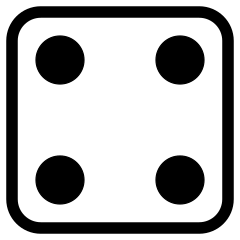
\includegraphics[height=0.9em]{figs/4.png} side of the die, making it 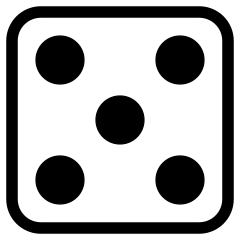
\includegraphics[height=0.9em]{figs/5.png}, and then added two dots on the 
\includegraphics[height=0.9em]{figs/1.png} side, making it 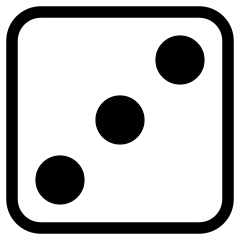
\includegraphics[height=0.9em]{figs/3.png}.
What is the probability that the outcome of the die is greater than $4$? Find the expectation and variance of the die.
\end{problem}
\medskip

\begin{problem}
    The world famous gambler Vardanik from Parakar proposes the following game of chance. You roll a fair die. If you roll $1$,  Vardanik pays you $\$25$. If you roll  $2$, 
Vardanik pays you \$$5$. If you roll $3$, you win nothing. If you roll $4$ or $5$, you must 
pay Vardanik \$$10$, and if you roll $6$, you must pay Vardanik \$15. Do you want to play? 
\end{problem}


\medskip 


% Yet another good one
% \begin{problem}
%     You draw one card from a 52-card deck of playing cards. If you pick a heart, you will win 
% \$10. If you pick a face card (i.e. Jack, Queen or King), which is not a heart, you win \$8. If you pick any other card, 
% you lose \$6. Do you want to play? Approximately how much would you win or lose after playing 1,000,000 times?
% \end{problem}


% 13
\begin{problem}
Let $X$ be a random variable with the PDF:
\[
f(x) = \begin{cases}
   2x, & 0 \le x \le 1 \\
   0, & \text{otherwise}
\end{cases}
\]

Find the expectation and variance of
\begin{enumerate}
   \item[a) ] $X$,
   \item[b) ] $2X$,
   \item[c) ] $2X + 7$. 
   
\end{enumerate}
\end{problem}
\medskip



% \begin{problem}[0.5 points]
% There are 1 green, 4 blue and 6 red balls in a box. If we randomly
% take out 3 balls, what is the probability that exactly 2 of them have
% different colors (e.g. 2 blue, 1 green)?

% \end{problem}
% \bigskip

% \bigskip

% \begin{problem}[0.5 points]
%     There are two strawberry-flavored, three caramel and two chocolate candies in the box. Two candies are randomly drawn from the box. What is the probability that one of them will be strawberry-flavored and the other one caramel or chocolate?
% \end{problem}
% \bigskip
% \begin{problem}[1 point]
% Ashot, Anush and Armen can hit the target with one shot with probabilities $0.8$, $0.75$ and $0.6$. They shot at the same time and one of them missed the target. What is the probability that it was Armen?
% \end{problem}
% \bigskip



% \bigskip


% \begin{problem}[1 point]
% In a certain town, 30\% of the people are conservatives, 50\% socialists and 20\% liberals. At the last election, 65\% of conservatives voted, 82\% of socialists and 50\% of liberals. A person from the town is selected at random, and states that she voted at the last election. What is
% the probability that she is a socialist?
% \end{problem}

% \bigskip

% \bigskip

% \bigskip

% \bigskip
% \begin{problem}[1 point]
%     Let $X$ be a continuous random variable with PDF
% \[
% f_X(x) = \begin{cases}
%     \frac{3}{x^4},& x \ge 1 \\
%     0,& \text{otherwise}
% \end{cases}
% \]

% Find the expectation and variance of $X$.
% \end{problem}
% \bigskip
\begin{problem}[\textbf{additional}]%[0.5 points]
    Let $X$ and $Y$ be two continuous random variables with uniform distribution on $(0,2)$. Find the expectation of $X+Y$.
\end{problem}

\medskip
% \begin{problem}
%     Nare and Arman both go to school at some random time between 9:00 and 9:30.
    
%     \begin{enumerate}
%         \item[a) ] What is the probability that Arman arrives sooner than Nare?
        
%         \item[b) ] If after arriving Arman waits another $5$ minutes after he enters, what is the probability that he meets Nare?
        
%     \end{enumerate} 
% \end{problem}
% \bigskip
\begin{problem}[\textbf{additional}]
    Let $X$ be a random variable with PDF
    \[
    f_X(x) = \begin{cases}
        ax^5,& \text{if }0\le x \le 3 \\
        0,& \text{otherwise}
    \end{cases}
    \]
where $a$ is an unknown constant. Can you find the value of $a$?
\end{problem}
